\documentclass{article} % For LaTeX2e

\usepackage{iclr2026_conference,times}
\input{math_commands.tex}

\usepackage{amsmath,amssymb}
\usepackage{graphicx}
\usepackage{booktabs}
\usepackage{hyperref}
\usepackage{url}

\graphicspath{{figures/}}

\title{Sketched Empirical-NTK Capability Fingerprints Predict\\
Fine-Tuning Transfer and Interference in Large Language Models}

% Anonymous submission: authors hidden until \iclrfinalcopy is uncommented.
\author{Anonymous authors\\Paper under double-blind review}

\begin{document}
\maketitle

\begin{abstract}
Fine-tuning a large language model on new data routinely improves one capability while
silently degrading others, but which capabilities will transfer and which will interfere
is usually discovered only after the (expensive) training run. We introduce a
\emph{capability fingerprint}: for each capability we CountSketch-compress the per-prompt
gradients of the answer cross-entropy with respect to a small, fixed parameter subset
($\sim$73M of 7.6B parameters), and predict capability-level transfer from the mean sketch
inner product between a candidate fine-tuning set and any held-out capability---\emph{before
any training is run}. The predictor is the empirical neural tangent kernel: to first order,
one gradient step on capability $i$ changes the loss on capability $j$ by
$-\eta\langle g_i, g_j\rangle$. Across four settings validated with one recipe and no
per-setting tuning---homogeneous long-context tasks (RULER), heterogeneous real skills (math
CoT, code, QA, retrieval, aggregation), a trainer whose updated parameters are \emph{disjoint}
from the sketched subset (LoRA on all layers), and a second model family (Llama-3.1-8B)---the
off-diagonal Spearman correlation between predicted kernel and measured $\Delta$CE is
$0.68$, $0.87$, $0.62$, and $0.69$ (all $p \le 0.004$). An ablation isolates what carries the
signal: gradient \emph{direction} is necessary, magnitude alone fails in three of four
settings, and representation (embedding) similarity---the standard ``similar data'' heuristic
for data selection---fails in all four and is significantly \emph{anti}-correlated in the
heterogeneous setting ($\rho=-0.62$). We also report an honest null: the self-gradient norm as
a test-time correctness signal is confidence-in-disguise (cross-validated $\Delta$AUC over
free logit baselines $\approx -0.002$/$-0.0001$). The fingerprint costs one backward pass and
4096 stored floats per prompt, enabling data selection, rehearsal targeting, and forgetting-risk
assessment at negligible cost.
\end{abstract}

\section{Introduction}
\label{sec:intro}

Fine-tuning is the dominant way to adapt a pretrained language model to a new task or
distribution, but it is a blunt instrument: gradient steps that improve the target skill also
perturb every other capability the model had, sometimes catastrophically. Practitioners
mitigate this with data selection, rehearsal of old data, and conservative learning rates, but
these decisions are made largely blind---the actual transfer and interference structure is
revealed only \emph{after} a training run, when the affected capabilities are re-evaluated.
A cheap, \emph{pre}-training-time estimate of ``if I train on this data, which capabilities
improve, which are damaged, and how strongly'' would directly inform data selection, tell us
which capabilities to rehearse, and quantify forgetting risk before committing compute.

First-order learning dynamics give a principled handle on this question. A single gradient step
on a sample changes the loss on any other sample by the inner product of their loss gradients:
the empirical neural tangent kernel (eNTK) \citep{jacot2018ntk,malladi2023kernel}. Aggregated
over a training set and an evaluation set, this inner product is a first-order prediction of
capability-level transfer. The obstacle is cost: full-parameter gradients of a 7--8B model are
enormous, and materializing them for every pairing of capabilities is infeasible. We remove the
obstacle with two choices---restrict gradients to a small fixed parameter subset, and compress
them with a single CountSketch projection \citep{charikar2002countsketch}---and show empirically
that the resulting low-dimensional \emph{fingerprint} preserves enough kernel geometry to
predict measured fine-tuning outcomes across model families and even when the trained parameters
differ from the sketched ones.

Our starting point was a diagnostic study of long-context ``rank demand'': we asked whether the
spectral structure that different long-context tasks induce in attention and hidden states
predicts correctness. It does not (Section~\ref{sec:results}, ablation): rank is task-intrinsic
and model-stable but adds no per-sample predictive value once entropy is controlled. In the same
data, per-prompt gradient (eNTK) features were the strongest signal. This negative$\rightarrow$positive
contrast pointed us away from activation space and toward gradient space, where first-order
training dynamics actually live.

\paragraph{Contributions.}
\begin{enumerate}
  \item \textbf{A cheap, pre-training-time predictor of fine-tuning transfer and interference.}
    Per capability we compute a fingerprint---CountSketch-compressed per-prompt answer-loss
    gradients on a fixed $\sim$73M-parameter subset (under 1\% of the model). The mean sketch inner
    product between a fine-tuning set and a held-out capability predicts that capability's
    measured $\Delta$CE after actual fine-tuning.
  \item \textbf{Validation across four settings} with the same recipe and no per-setting tuning:
    homogeneous long-context (RULER), heterogeneous real capabilities, a LoRA trainer whose
    updated parameters are disjoint from the sketched subset, and a second model family
    (Llama-3.1-8B). Off-diagonal Spearman between predicted kernel and measured $\Delta$CE:
    $0.68, 0.87, 0.62, 0.69$ (all $p \le 0.004$).
  \item \textbf{An ablation isolating the ingredient that carries transfer structure.} Gradient
    magnitude alone fails in three of four settings; embedding similarity fails in four of four
    and is significantly anti-correlated in the heterogeneous setting ($\rho=-0.62$). Gradient
    \emph{direction} is necessary; the full inner product is best everywhere.
  \item \textbf{A motivating rank-demand diagnostic} showing that attention/hidden-state spectral
    structure is task-intrinsic and model-stable but has no incremental per-sample predictive
    value for correctness, whereas per-prompt gradient features do---the useful geometry lives in
    gradient space.
  \item \textbf{An honest null.} The self-gradient norm as a test-time correctness signal adds
    nothing over free confidence baselines (CV $\Delta$AUC $\approx -0.002$); raw gradient norms
    are confidence in disguise, and it is the \emph{kernel} structure, not the norm, that carries
    training-relevant information.
\end{enumerate}

\section{Related Work}
\label{sec:related}

\paragraph{NTK and linearized fine-tuning.}
The neural tangent kernel~\citep{jacot2018ntk} shows that sufficiently wide networks
train as their first-order Taylor expansion about initialization, with dynamics governed
by a fixed gradient-inner-product kernel~\citep{lee2019wide,arora2019exact}; the
\emph{empirical} NTK measured at finite width is a widely used practical surrogate,
and fast approximations make it computable for large models~\citep{novak2022fast,mohamadi2023entk,fort2020deep}.
Closest to us, \citet{malladi2023kernel} extend this lens to \emph{fine-tuning} pretrained
language models, arguing (and empirically verifying, including an extension to Adam via
Tensor Programs) that fine-tuning frequently behaves kernel-like, and a recent theoretical
line makes the linearization argument explicit for LLMs~\citep{afzal2026linearization}.
These works establish \emph{that} an eNTK describes LLM fine-tuning on a single task. We take
the complementary, constructive step: we \emph{use} the eNTK predictively \emph{across}
capabilities, turning the first-order transfer identity
$\Delta L(s_j)\approx-\eta\langle g(s_i),g(s_j)\rangle$ into a pre-training-time forecast of
which held-out capabilities a candidate fine-tuning set will improve or damage, validated
against \emph{measured} $\Delta$CE at 7--8B scale.

\paragraph{Gradient-based data attribution and influence.}
Influence functions attribute a model's behavior to individual training points via
gradient and inverse-Hessian information~\citep{koh2017influence}, with scalable variants
that trace gradient descent~\citep{pruthi2020tracin}, exploit random projections of
per-example gradients~\citep{park2023trak}, or approximate the inverse Hessian for
LLM-scale valuation~\citep{grosse2023influence,choe2024logra,kwon2024datainf,ilyas2022datamodels}.
This literature is \emph{backward-looking}: it explains the predictions of a model that has
\emph{already} been trained, and typically requires a per-query solve or Hessian
approximation. Our object differs in three ways: (i) we predict the effect of \emph{future}
fine-tuning from \emph{base-model} gradients, before any training; (ii) we need no Hessian
inversion or optimizer trajectory---a single fixed CountSketch per prompt supports all
future capability pairings; and (iii) our unit of prediction is a \emph{capability
distribution}, not an individual training point, yielding a full transfer/interference
matrix.

\paragraph{Gradient-based data selection and transferability estimation.}
The machinery closest to ours appears in gradient-based data selection.
\textsc{Less}~\citep{xia2024less} selects instruction-tuning data by projecting
optimizer-aware (Adam) gradients collected \emph{along a training trajectory} and matching
them to a \emph{fixed target task}; NTK-Selector~\citep{wang2026ntkselector} concurrently
uses random-projected NTK scores at initialization to mine auxiliary data for a
\emph{single} low-resource domain. We share the low-dimensional gradient-feature idea but
differ in goal and validation: rather than ranking data for one target, we predict the
\emph{entire} cross-capability transfer \emph{and} interference matrix from base-model
gradients and check it against measured $\Delta$CE, including the case where the trained
parameters (all-layer LoRA) are \emph{disjoint} from the sketched subset. A parallel thread
estimates \emph{task affinity} from gradients for multi-task grouping---TAG measures how one
task's gradient step changes another's loss~\citep{fifty2021tag}, Grad-TAG fits a logistic
surrogate on projected gradients to predict combined-task loss~\citep{li2024gradtag}, and
earlier work groups tasks by cooperation/competition~\citep{standley2020which}---but these
target \emph{which tasks to co-train} (positive transfer for grouping), operate during or
across training runs, and are demonstrated below LLM scale. Transferability metrics such as
Task2Vec~\citep{achille2019task2vec}, TaskEmb~\citep{vu2020exploring},
LEEP~\citep{nguyen2020leep}, LogME~\citep{you2021logme}, and the
H-score~\citep{bao2019hscore,zamir2018taskonomy} likewise \emph{embed} tasks or score
source-model reusability; notably Task2Vec fingerprints a task with Fisher-weighted
gradients, but for meta-learning similarity---it does not predict a measured fine-tuning
$\Delta$CE transfer matrix, and uses a different gradient object than our pairwise eNTK
inner products.

\paragraph{Forgetting and task interference.}
Fine-tuning LLMs degrades pretraining capabilities~\citep{luo2023empirical,kotha2024understanding},
extending classic studies of forgetting~\citep{kirkpatrick2017ewc,toneva2019empirical}, and
is commonly mitigated by regularization or rehearsal/replay~\citep{scialom2022finetuned,huang2024selfsynth}.
In weight space, task vectors interfere when models are merged, motivating sign- and
magnitude-based conflict resolution~\citep{ilharco2023task,yadav2023ties}; in gradient space,
multi-task optimization identifies conflicting (negatively aligned) gradients and surgically
removes the conflict~\citep{yu2020pcgrad,wang2021gradvaccine,du2018adapting}. The work
theoretically nearest to our interference claim is \citet{doan2021ntkoverlap}, who show that
catastrophic forgetting between two tasks grows with their NTK overlap and formalize task
similarity through an NTK overlap matrix, complemented by representational analyses of what
drives forgetting~\citep{ramasesh2021anatomy}. That line is theoretical, is developed for
two-task continual learning in vision, and prescribes an \emph{intervention} (orthogonal
gradient descent) rather than a validated quantitative forecast. We instead \emph{measure}
the full signed transfer/interference matrix induced by real fine-tuning of a 7--8B LLM and
show that a cheap sketched-eNTK kernel predicts it---capturing both damage (positive
$\Delta$CE) and benefit (negative $\Delta$CE), across heterogeneous real capabilities and two
model families---which in turn enables rehearsal targeting. This complements our companion
function-space analysis of when such forgetting is low-rank~\citep{hidekel2026forgetting}.

\paragraph{Sketching gradients.}
We compress each gradient with CountSketch~\citep{charikar2002countsketch}, an unbiased
inner-product-preserving projection in the Johnson--Lindenstrauss family~\citep{johnson1984extensions}
also known as the hashing trick~\citep{weinberger2009feature}; the same random-projection
principle underlies gradient attribution~\citep{park2023trak} and selection~\citep{xia2024less}.
Our use is distinctive in that one fixed sketch per prompt is reused across \emph{all}
capability pairings to reconstruct the Gram matrix without ever materializing gradients.
Finally, we report an honest negative result: the \emph{norm} of a self-generated answer's
gradient---a natural test-time confidence signal in the spirit of gradient-based
uncertainty~\citep{lee2020gradients}---adds nothing over free logit-based baselines, underscoring
that the predictive content lives in the \emph{inner-product structure} of the kernel, not in
gradient magnitude.


\section{Mathematical Background}
\label{sec:background}

\paragraph{Teacher-forced answer loss and per-sample gradient.}
Let $f_\theta$ be a causal language model with parameters $\theta$. A \emph{capability} $c$ is a
distribution over $(x,y)$ pairs, where $x$ is a prompt and $y=(y_1,\dots,y_T)$ its reference
answer. For a sample $s=(x,y)$ the teacher-forced answer loss is the cross-entropy of $y$ under
the model conditioned on $x$,
\begin{equation}
  L(s;\theta) \;=\; -\frac{1}{T}\sum_{t=1}^{T} \log f_\theta\!\left(y_t \mid x, y_{<t}\right),
\end{equation}
computed only over answer tokens (the prompt is masked). We restrict attention to a fixed
parameter subset $S\subseteq\theta$ and define the per-sample gradient
$g(s) = \nabla_{\theta_S} L(s;\theta) \in \mathbb{R}^{|S|}$.

\paragraph{The prediction we make.}
The quantity we want, \emph{before running any training}, is the change in the loss on a
held-out capability $j$ caused by fine-tuning on capability $i$. Fine-tuning displaces the
parameters from $\theta_S$ to $\theta_S+\Delta\theta_i$, and the loss on any sample $s_j$ changes
by a Taylor expansion in that displacement. The leading term is the inner product between $s_j$'s
loss gradient and the update direction; the update direction is itself a (preconditioned) sum of
the \emph{training} gradients. The core claim of the method is that this leading term is well
approximated by --- and can be predicted from --- the gradient inner products
$\langle g(s), g(s')\rangle$ measured at the \emph{base} model, without ever taking the training
step. Below we make the approximation and its error terms explicit.

\paragraph{One gradient step: the leading term and the curvature it drops.}
Take a single gradient-descent step of size $\eta$ on sample $s_i$,
$\theta_S \leftarrow \theta_S - \eta\, g(s_i)$, and expand the loss on a second sample $s_j$ to
second order in the displacement $-\eta g(s_i)$:
\begin{equation}
\begin{split}
  \Delta L(s_j)
  \;=\; L\!\big(s_j;\theta - \eta g(s_i)\big) - L(s_j;\theta)
  \;=\;\; & \underbrace{-\,\eta\,\big\langle g(s_i),\, g(s_j)\big\rangle}_{\text{first order (the eNTK)}}
  \;+\; \underbrace{\tfrac{1}{2}\,\eta^2\, g(s_i)^{\!\top} H_j\, g(s_i)}_{\text{curvature}} \\[2pt]
  & +\; O\!\big(\eta^3 \|g(s_i)\|^3\big),
\end{split}
  \label{eq:secondorder}
\end{equation}
where $H_j = \nabla^2_{\theta_S} L(s_j;\theta)$ is the Hessian of the loss on $s_j$ at the base
parameters. The neglected term is therefore \emph{not} a bare $O(\eta^2)$ with a universal
constant: its size is set by the curvature and the \emph{squared gradient norm}, and is bounded by
\begin{equation}
  \Big|\tfrac{1}{2}\eta^2\, g(s_i)^{\!\top} H_j\, g(s_i)\Big|
  \;\le\; \tfrac{1}{2}\,\eta^2\,\|H_j\|_2\,\|g(s_i)\|^2 .
  \label{eq:curvbound}
\end{equation}
The first-order (eNTK) prediction dominates precisely when
$\eta\,\|H_j\|_2\,\|g(s_i)\|^2 \ll \big|\langle g(s_i),g(s_j)\rangle\big|$, i.e.\ for small learning
rate and mild curvature along the update direction. Because we validate by \emph{rank} agreement,
we need only that this curvature correction not reorder the capability pairs --- a substantially
weaker condition than it being negligible in magnitude.

\paragraph{A whole fine-tuning run.}
Fine-tuning on $T_i$ is a sequence of such steps. Writing the net displacement as
$\Delta\theta_i$, the second-order expansion of the loss on $s_j$ is
\begin{equation}
  \Delta L(s_j) \;=\; \big\langle g(s_j),\, \Delta\theta_i\big\rangle
  \;+\; \tfrac{1}{2}\,\Delta\theta_i^{\!\top} H_j\, \Delta\theta_i \;+\; O\!\big(\|\Delta\theta_i\|^3\big).
  \label{eq:runexpand}
\end{equation}
For a (possibly preconditioned) descent trajectory,
$\Delta\theta_i = -\eta\sum_{t} P_t\, g^{(t)}$, where $g^{(t)}$ is the minibatch gradient at step
$t$ and $P_t$ is the optimizer's preconditioner ($P_t=I$ for SGD; a diagonal matrix for Adam).
Two approximations reduce the leading term to a base-model kernel: \textbf{(A1)~trajectory
stability} --- over a short run the gradients rotate little, $g^{(t)}\approx g$ evaluated at the
base $\theta$; and \textbf{(A2)~scalar preconditioning} --- $P_t\approx c\,I$, discarding Adam's
per-coordinate reweighting. Under (A1)--(A2),
$\Delta\theta_i \approx -\eta c\sum_{s\in T_i} g(s)$, so
$\langle g(s_j),\Delta\theta_i\rangle \approx -\eta c\sum_{s\in T_i}\langle g(s_j), g(s)\rangle$.
Averaging over the train set $T_i$ and eval set $E_j$ gives the predicted transfer matrix
\begin{equation}
  K[i,j] \;=\; \frac{1}{|T_i|\,|E_j|}\sum_{s\in T_i}\sum_{s'\in E_j}
             \big\langle g(s),\, g(s')\big\rangle,
  \qquad
  \text{predicted } \Delta\mathrm{CE}[i,j] \;\propto\; -\,K[i,j].
  \label{eq:kernel}
\end{equation}
Positive $K[i,j]$ predicts that training on $i$ \emph{reduces} the loss on $j$ (transfer);
negative $K[i,j]$ predicts an \emph{increase} (interference).

\paragraph{What the prediction drops, and why rank survives it.}
Equation~\eqref{eq:kernel} is exact only in the limit of a single infinitesimal step with
identity preconditioner. Four error sources separate it from the measured $\Delta$CE, and it is
worth naming them because they set the regime of validity: \textbf{(1)~curvature} --- the
$\tfrac12\Delta\theta_i^\top H_j\Delta\theta_i$ term of \eqref{eq:runexpand}, of order
$\|H_j\|_2\,\|\Delta\theta_i\|^2$, which grows with $\eta^2$ and with the square of the training
horizon; \textbf{(2)~trajectory drift} --- the error in (A1), which grows with $\eta$ times the
number of steps; \textbf{(3)~preconditioning} --- the error in (A2), since our actual optimizer is
Adam, whose diagonal reweighting is not a global scalar; and \textbf{(4)~sketching variance}
(\S\ref{sec:method}), of order $1/m$. All four leave the \emph{sign} and coarse ordering of
$K[i,j]$ intact as long as $\eta$ and the horizon are small, which is why we report Spearman rank
and Pearson agreement with measured $\Delta$CE rather than claiming an exact magnitude match, and
why the constant of proportionality (absorbing $\eta$, $c$, and step count) is left free. The
horizon-scaling experiment (\S\ref{sec:conclusion}, future work) probes exactly when errors
(1)--(2) grow large enough to degrade the rank prediction.

\paragraph{Empirical neural tangent kernel.}
The Gram matrix $\langle g(s), g(s')\rangle$ is the empirical NTK of $f_\theta$ contracted with
the loss Jacobians, evaluated at the base parameters \citep{jacot2018ntk,malladi2023kernel}.
Unlike the infinite-width NTK it is not constant along training, but for the short fine-tuning
horizons of interest the first-order term of \eqref{eq:runexpand} is the one that governs
transfer, and its cross-capability structure is exactly what $K$ estimates. Our method is a
scalable estimator of this Gram matrix and a study of how well its structure predicts real
fine-tuning outcomes.

\paragraph{CountSketch and inner-product preservation.}
Materializing $g(s)\in\mathbb{R}^{|S|}$ for every sample is wasteful when only inner products
are needed. CountSketch \citep{charikar2002countsketch} is a sparse random projection
$\Phi:\mathbb{R}^{|S|}\to\mathbb{R}^{m}$ defined by two fixed hash functions: a bucket
$h:\{1,\dots,|S|\}\to\{1,\dots,m\}$ and a sign $\sigma:\{1,\dots,|S|\}\to\{-1,+1\}$, with
$(\Phi g)_b = \sum_{k:h(k)=b}\sigma(k)\,g_k$. Drawn once (fixed seed) and shared across all
samples, $\Phi$ is an unbiased estimator of inner products,
\begin{equation}
  \mathbb{E}\big[\langle \Phi g,\, \Phi g'\rangle\big] \;=\; \langle g,\, g'\rangle,
  \qquad
  \mathrm{Var}\big[\langle \Phi g,\, \Phi g'\rangle\big] \;=\; O\!\left(\tfrac{1}{m}\,\|g\|^2\,\|g'\|^2\right),
  \label{eq:countsketch}
\end{equation}
the sign flips cancelling cross terms in expectation and the variance decaying as $1/m$. With
$m=4096$ the standard deviation of a normalized inner product is $O(1/\sqrt{m})\approx 1.6\%$;
because our Gram entries are \emph{averaged} over $|T_i|\times|E_j| \ge 30\times 30$ pairs, the
per-cell error is suppressed by a further factor of $\sqrt{|T_i||E_j|}$, which is why $m=4096$
suffices to recover the capability-level kernel structure at $16$\,KB per prompt.

\paragraph{Why a parameter subset still captures kernel structure.}
Restricting $S$ to a small set of tensors loses parameters but not, empirically, the geometry
that matters: gradient directions are strongly shared across the network, so a subset's Gram
matrix is a good proxy for the full one. Section~\ref{sec:results} makes this concrete: in the
LoRA setting the trained parameters (low-rank adapters on \emph{all} layers) are disjoint from
the sketched subset (q/v projections of five layers), yet the subset fingerprint still predicts
the measured transfer, evidence that we are reading a network-wide gradient geometry rather than
memorizing exactly what we train.

\section{Method}
\label{sec:method}

\paragraph{Parameter subset.}
$S$ is the query and value projections (\texttt{q\_proj}, \texttt{v\_proj}) of five layers at
depth fractions $\{0,\tfrac14,\tfrac12,\tfrac34,1\}$---approximately $73$M parameters of a $7.6$B model ($0.97\%$; $105$M for Llama-3.1-8B). It is fixed once per model and never tuned per task.

\paragraph{Sketched fingerprints.}
For each sample we run one forward and one backward pass on the frozen model with gradients
enabled only on $S$, apply $\Phi$ per parameter tensor and sum, and store the resulting
$m=4096$-dimensional sketch. The fingerprint of a capability $c$ is the set
$\{\Phi g(s): s\in c\}$, $16$\,KB per prompt. No training is performed and no labels beyond the
reference answers already needed for evaluation are used. With gradient checkpointing the
procedure fits generation-scale memory.

\paragraph{Prediction protocol.}
Given capabilities $c_1,\dots,c_n$ with seed-disjoint train sets $T_i$ and eval sets $E_j$:
(1)~sketch all train and eval samples once with the same $\Phi$;
(2)~form the predicted transfer matrix $K$ via \eqref{eq:kernel} from sketch inner products;
(3)~for ground truth, fine-tune the model on $T_i$ alone, measure $\Delta$CE on every $E_j$,
restore weights, and repeat for each $i$;
(4)~score by Spearman and Pearson correlation between $-K$ and measured $\Delta$CE over all
$(i,j)$ pairs, and---the stricter test---over \emph{off-diagonal pairs only}, which removes the
easy ``training on $X$ helps $X$'' diagonal signal and isolates cross-capability
transfer/interference.

\paragraph{Validation settings.}
We validate the same recipe on four axes (Table~\ref{tab:settings}). The LoRA setting is the key
robustness axis: the fingerprint is computed on five layers' q/v while training updates rank-16
LoRA adapters on the q/v of \emph{all} layers, so the prediction can only succeed if gradient
geometry is shared across the network rather than because we sketch exactly what we train.

\begin{table}[t]
\centering
\small
\caption{Validation settings. All use $n_{\text{train}}=32$, $n_{\text{eval}}=30$ per capability,
3 epochs; outcome is gold-answer $\Delta$CE.}
\label{tab:settings}
\resizebox{\textwidth}{!}{%
\begin{tabular}{@{}llll@{}}
\toprule
Setting & What it tests & Trainer & Capabilities \\
\midrule
RULER $5\times5$ & base validity & Adam on subset $S$ & 5 RULER families @1024 \\
Heterogeneous    & real, dissimilar skills & Adam on subset $S$ & GSM8K CoT, MBPP, SQuAD QA, needle, aggregation \\
LoRA             & trained $\ne$ sketched params & rank-16 LoRA, all q/v layers & 5 RULER families \\
Llama-3.1-8B     & model-family generality & Adam on subset $S$ & 5 RULER families \\
\bottomrule
\end{tabular}}
\end{table}

\paragraph{Trainer details.}
Fine-tuning fp16 weights directly with Adam \citep{kingma2015adam} destroys the model; we keep
fp32 master copies of the trainable parameters, apply dynamic loss scaling, and skip any update
whose gradients are non-finite (Appendix~\ref{app:trainer}). Learning rate is $2\times10^{-5}$
for subset training and $2\times10^{-4}$ for LoRA. Capabilities and models are drawn from RULER
\citep{hsieh2024ruler}, GSM8K \citep{cobbe2021gsm8k}, MBPP \citep{austin2021mbpp}, SQuAD
\citep{rajpurkar2016squad}, Qwen2.5-7B-Instruct \citep{qwen2p5}, and Llama-3.1-8B-Instruct
\citep{llama3}.

\paragraph{Baselines.}
Against the same measured $\Delta$CE matrices we compare four pre-training predictors:
\textbf{ntk\_kernel} (ours, mean $\langle g,g'\rangle$, direction $\times$ magnitude);
\textbf{ntk\_cos} (mean cosine, direction only);
\textbf{grad\_magnitude} (mean $\|g\|\,\|g'\|$, magnitude only); and
\textbf{embed\_cos} (mean cosine of last-hidden-state mean-pooled prompt embeddings---the
standard representation-similarity ``similar data'' heuristic used in embedding-based data
selection).

\section{Results}
\label{sec:results}

\paragraph{The kernel predicts measured transfer in all four settings.}
Table~\ref{tab:main} reports, for our predictor, the Spearman and Pearson correlation between
$-K$ and measured $\Delta$CE over all $25$ $(i,j)$ pairs, and the off-diagonal Spearman over the
$20$ cross-capability pairs. Off-diagonal agreement is $0.68$/$0.87$/$0.62$/$0.69$
(RULER/hetero/LoRA/Llama), all significant at $p\le 0.004$; pooled Pearson over all pairs is
$0.98$/$0.92$/$0.88$/$0.75$. Figure~\ref{fig:scatter} shows the corresponding scatter plots, with
off-diagonal points highlighted: the predicted ordering tracks the measured $\Delta$CE across
more than three orders of magnitude of kernel scale, and---critically---does so on the
off-diagonal, where the diagonal ``self-transfer'' shortcut is removed.

\begin{table}[t]
\centering
\small
\caption{Main result: correlation of the predicted kernel ($-K$) with measured $\Delta$CE, for
the \textbf{ntk\_kernel} predictor. ``All'' = 25 pairs; ``off-diag'' = 20 cross-capability pairs
(stricter). $p$-values as reported; $<\!10^{-4}$ shown for machine-zero.}
\label{tab:main}
\begin{tabular}{@{}lcccc@{}}
\toprule
 & Spearman (all) & Pearson (all) & Spearman (off-diag) & $p$ (off-diag) \\
\midrule
RULER (subset) & $0.79$ & $0.98$ & $0.68$ & $0.001$ \\
Heterogeneous  & $0.91$ & $0.92$ & $0.87$ & $<\!10^{-4}$ \\
LoRA           & $0.78$ & $0.88$ & $0.62$ & $0.004$ \\
Llama-3.1-8B   & $0.82$ & $0.75$ & $0.69$ & $0.0007$ \\
\bottomrule
\end{tabular}
\end{table}

\begin{figure}[t]
\centering
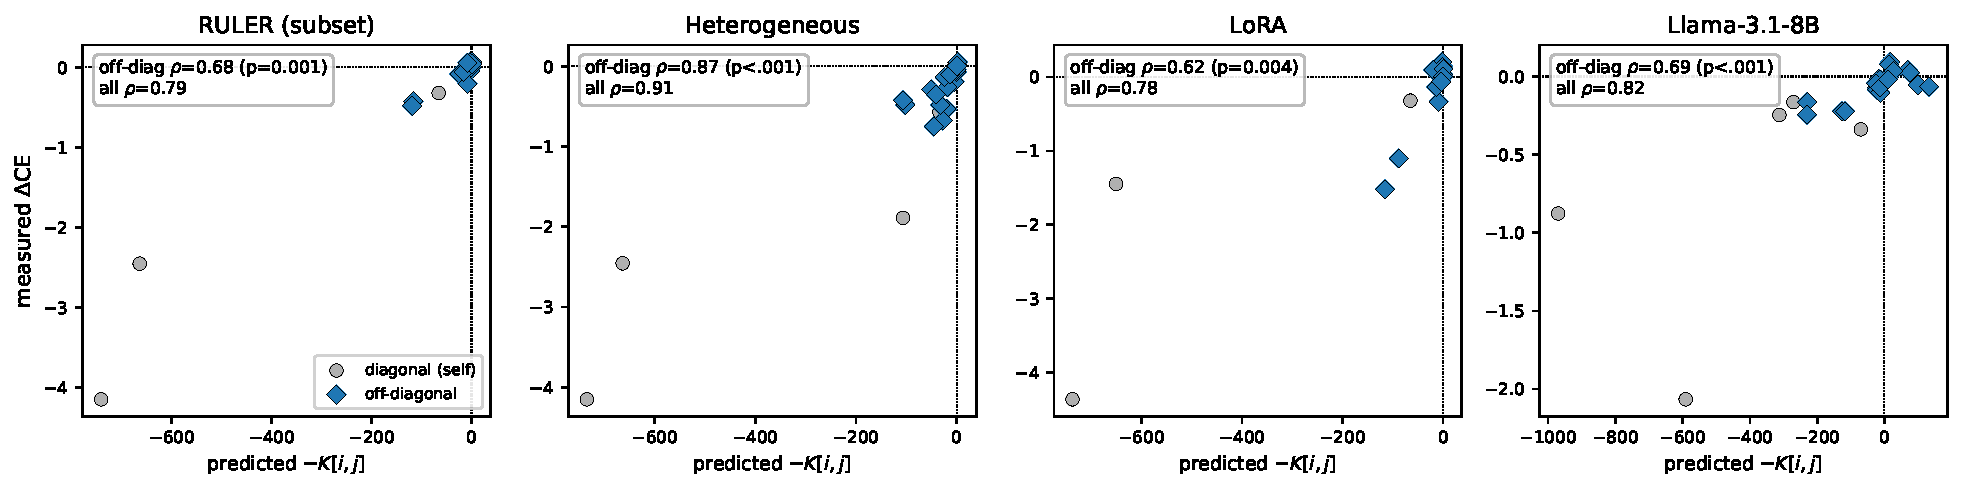
\includegraphics[width=\textwidth]{fig_scatter_4panel.pdf}
\caption{Predicted kernel ($-K[i,j]$, $x$) vs.\ measured $\Delta$CE ($y$) across the four
settings. Grey circles are diagonal (self) pairs, blue diamonds off-diagonal (cross-capability)
pairs. Off-diagonal Spearman $\rho$ (the stricter score) and all-pairs $\rho$ annotated. The
predicted kernel orders the measured loss changes across the full range, including the
off-diagonal where the self-transfer shortcut is absent.}
\label{fig:scatter}
\end{figure}

\paragraph{Predicted and measured matrices agree cell by cell.}
Figure~\ref{fig:heatmaps} places the measured $\Delta$CE matrix beside the predicted $-K$ matrix
for the heterogeneous setting under a common row/column order and a diverging colormap centered
at zero. The two share the same block structure: large negative diagonal (self-training helps),
strong transfer among the language capabilities (GSM8K, MBPP, QA mutually reduce loss), and
near-zero coupling to the retrieval capability (needle), whose row and column are close to zero
in both matrices. This heterogeneous setting is where the method is most useful and also where it
is strongest ($0.87$ off-diagonal), because real capabilities span the widest range of gradient
geometry.

\begin{figure}[t]
\centering
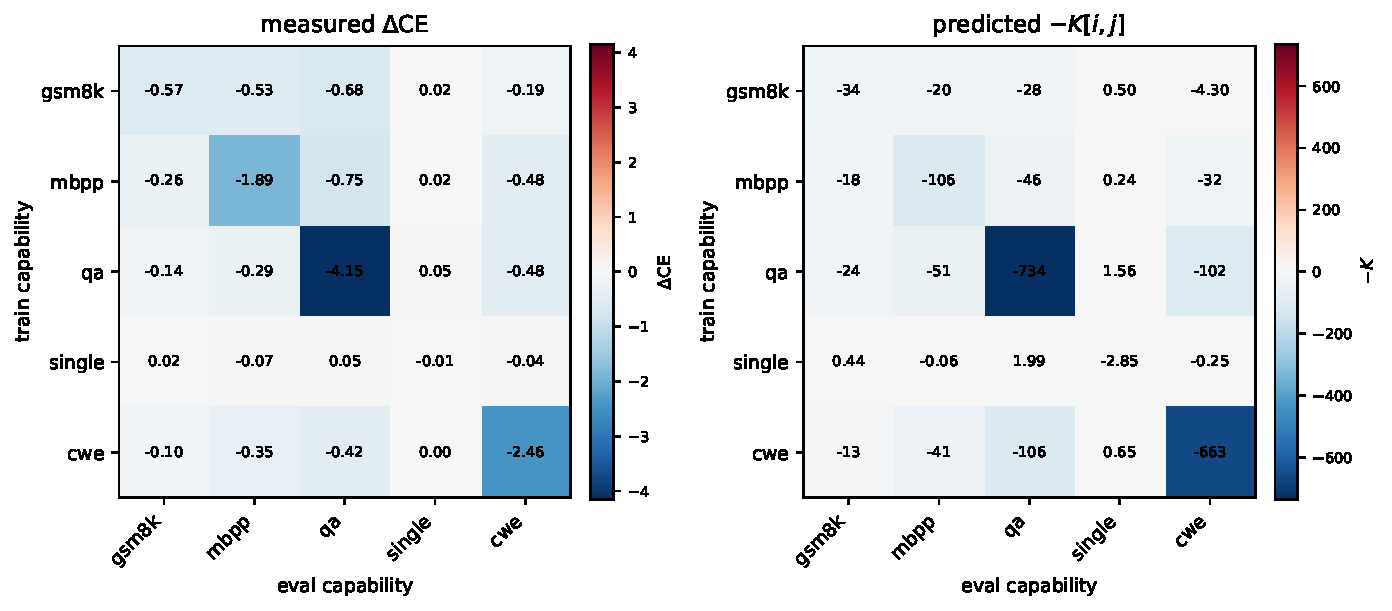
\includegraphics[width=0.92\textwidth]{fig_heatmaps_hetero.pdf}
\caption{Heterogeneous setting: measured $\Delta$CE (left) and predicted $-K$ (right), same
row/column order (train capability $\times$ eval capability), diverging colormap centered at
zero. The block structure matches: strong mutual transfer among GSM8K/MBPP/QA, near-zero
coupling to needle retrieval, large negative diagonal.}
\label{fig:heatmaps}
\end{figure}

\paragraph{Protocol note.}
All $\Delta$CE values are gold-answer cross-entropy changes measured by fine-tuning on a single
capability's train set and re-evaluating every capability (Section~\ref{sec:method}). Accuracy
deltas are tracked as a secondary outcome but are noisy at $n_{\text{eval}}=30$
(Appendix~\ref{app:tables}); we therefore report $\Delta$CE, the smoother first-order quantity
that the theory predicts.

\section{Ablation}
\label{sec:ablation}

\paragraph{What carries the transfer structure?}
Table~\ref{tab:baselines} and Figure~\ref{fig:baselines} compare the four predictors by
off-diagonal Spearman across the four settings. Three findings are consistent. \emph{(i)~Direction
is necessary.} The full kernel (ntk\_kernel) is the best predictor everywhere, with cosine
(ntk\_cos, direction only) close behind---the two dominate every other predictor in every
setting. \emph{(ii)~Magnitude alone is not enough.} grad\_magnitude collapses to non-significant
in three of four settings ($\rho=0.25$, $0.28$, $0.09$; $p>0.05$); it works only in the
heterogeneous setting, where capability-scale differences happen to align with transfer.
\emph{(iii)~Representation similarity fails.} embed\_cos---the standard heuristic that
``representationally similar data transfers''---is useless or actively misleading: it is
non-significant in the LoRA and Llama settings, and significantly \emph{anti}-correlated in the
heterogeneous setting ($\rho=-0.62$, $p=0.003$). Representationally similar prompts do not predict
training-time transfer; the gradient inner product does. (The RULER embedding baseline is omitted:
embeddings were not stored for that run.)

\begin{table}[t]
\centering
\small
\caption{Baseline shootout: off-diagonal Spearman $\rho$ vs.\ measured $\Delta$CE
($p$ in parentheses; \textit{n.s.} $=p>0.05$; ``---'' $=$ no data). Direction-carrying predictors
(top two rows) dominate; magnitude and embedding similarity fail in most settings.}
\label{tab:baselines}
\begin{tabular}{@{}lcccc@{}}
\toprule
Predictor & RULER & Heterogeneous & LoRA & Llama \\
\midrule
\textbf{ntk\_kernel (ours)} & $\mathbf{0.68}$ ($.001$) & $\mathbf{0.87}$ ($<\!10^{-4}$) & $\mathbf{0.62}$ ($.004$) & $\mathbf{0.69}$ ($.0007$) \\
ntk\_cos                    & $0.67$ ($.001$) & $0.79$ ($<\!10^{-4}$) & $0.55$ ($.012$) & $0.59$ ($.006$) \\
grad\_magnitude             & $0.25$ (\textit{n.s.}) & $0.80$ ($<\!10^{-4}$) & $0.28$ (\textit{n.s.}) & $0.09$ (\textit{n.s.}) \\
embed\_cos                  & --- & $-0.62$ ($.003$) & $-0.30$ (\textit{n.s.}) & $0.02$ (\textit{n.s.}) \\
\bottomrule
\end{tabular}
\end{table}

\begin{figure}[t]
\centering
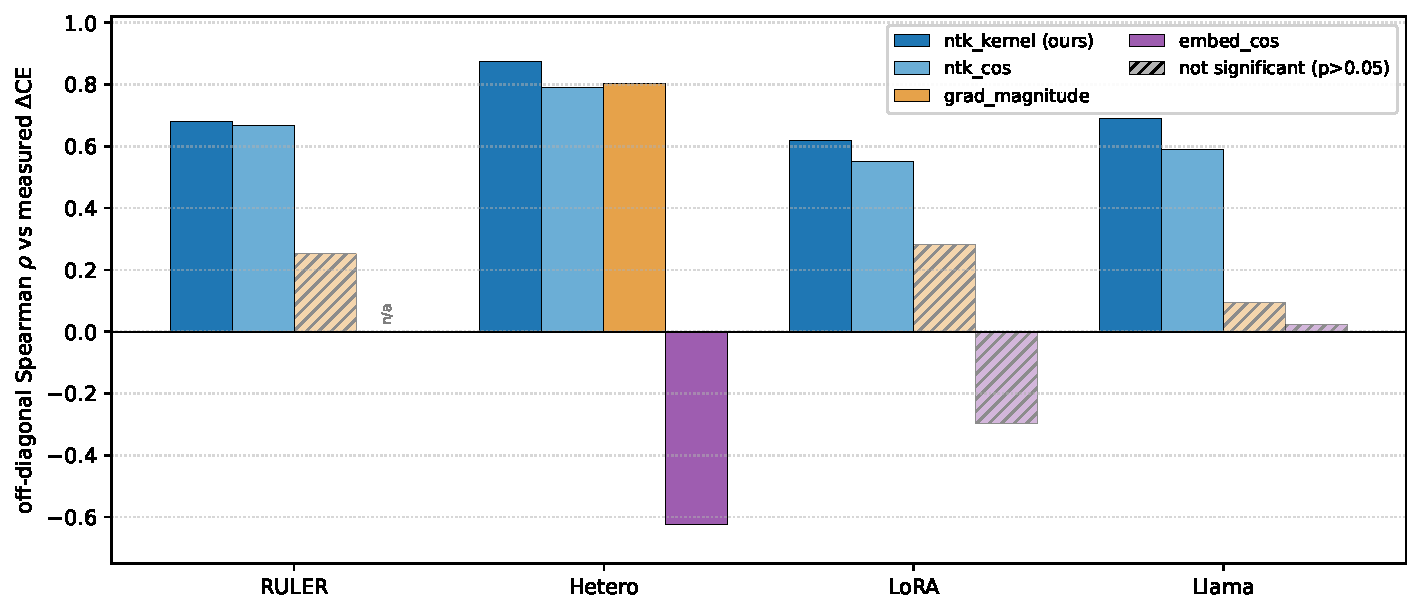
\includegraphics[width=0.88\textwidth]{fig_baselines.pdf}
\caption{Off-diagonal Spearman per predictor across the four settings. Hatched, translucent bars
are not significant ($p>0.05$); ``n/a'' marks the missing RULER embedding baseline. The
inner-product and cosine predictors (blue) are the only ones that are significant everywhere;
embedding similarity (purple) is negative where it is significant.}
\label{fig:baselines}
\end{figure}

\paragraph{LoRA vs.\ subset: trained $\ne$ sketched parameters.}
The LoRA setting is a robustness test, not merely a fourth dataset: the fingerprint is sketched
on the q/v projections of five layers, while training updates low-rank adapters on the q/v of all
layers---disjoint parameter sets. The predictor nonetheless attains $0.62$ off-diagonal Spearman
($p=0.004$) and $0.88$ pooled Pearson, only modestly below the matched-parameter RULER setting.
This supports the claim of Section~\ref{sec:background}: the fingerprint reads a network-wide
gradient geometry, so the sketched subset need not coincide with the trained parameters.

\paragraph{The self-gradient null.}
A tempting simpler idea is to use the gradient norm of the model's \emph{own generated} answer as
a test-time correctness signal. It fails. On $n\!=\!1000$ (Qwen) and $983$ (Llama) RULER samples,
self-gradient-norm AUC for predicting correctness is $0.78$/$0.76$, well below free logit
baselines: answer cross-entropy $0.90$/$0.89$ and mean-token entropy $0.90$/$0.91$
(Figure~\ref{fig:selfgrad}). Crucially, in a $5$-fold cross-validated logistic regression, adding
the gradient norm on top of the confidence baselines changes AUC by $-0.0016$ (Qwen) and
$-0.0001$ (Llama)---no incremental value. Gradient \emph{norms} are confidence in disguise; only
the \emph{kernel} (inner-product structure across samples) carries information not already in the
logits. This is the cautionary counterpart to the main result: the norm is not the signal, the
geometry is.

\begin{figure}[t]
\centering
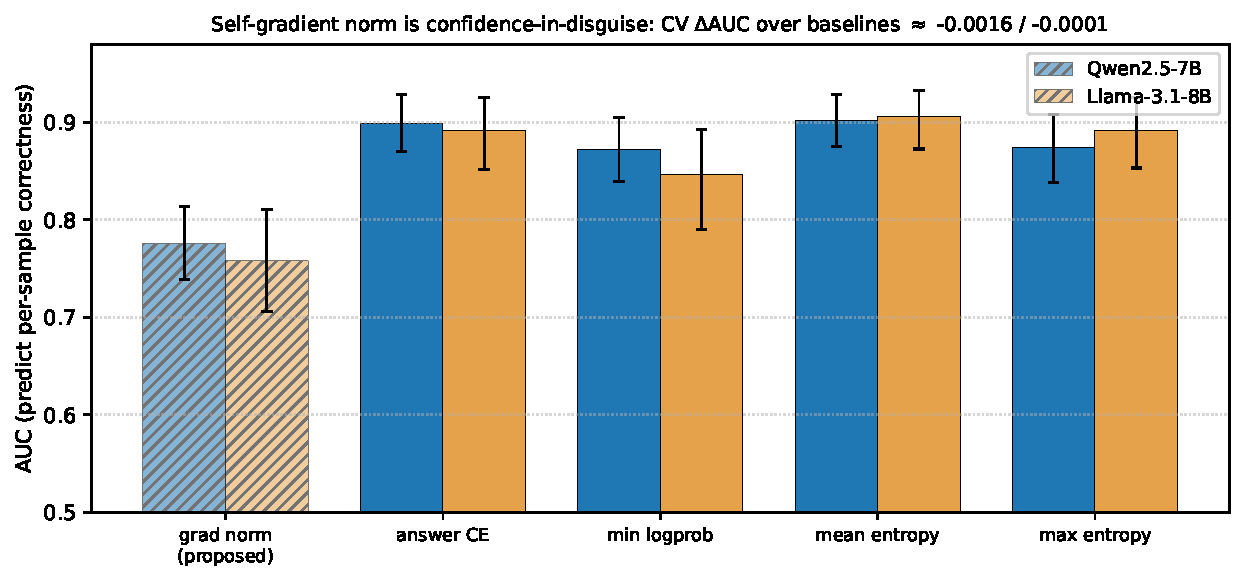
\includegraphics[width=0.82\textwidth]{fig_selfgrad_null.pdf}
\caption{Self-gradient null. Correctness-prediction AUC (with 95\% CIs) for the proposed
self-gradient norm (hatched) vs.\ free confidence baselines, on both models. The gradient norm is
the weakest predictor and adds cross-validated $\Delta$AUC $\approx -0.002$/$-0.0001$ on top of
the baselines.}
\label{fig:selfgrad}
\end{figure}

\paragraph{The rank-demand null (motivation evidence).}
The study that motivated the method is itself a null that points to gradient space. On five RULER
families at context lengths 1k--8k ($1000$ samples per model), hidden-state effective rank is
task-intrinsic and orders the families near-identically across Qwen and Llama
(Figure~\ref{fig:rank}), and the ordering is \emph{not} the attention-entropy ordering, so it is
not an entropy artifact. Yet in $5$-fold cross-validated logistic regression predicting
correctness, adding rank features on top of context length, family, and entropy changes AUC by
$-0.002$ (Qwen) and $+0.002$ (Llama)---an in-sample gain of $+0.010$ that vanishes under
cross-validation, i.e.\ pure overfit. In the same runs, per-prompt eNTK features showed exactly
the structure activation-space metrics lacked: within-family gradient cosine similarity is
$0.21$/$0.41$ (Qwen/Llama) versus $0.02$/$0.05$ across families, and self-kernel norms span
hundreds-fold across families. Prompts from the same capability occupy a tight cone in gradient
space while different capabilities are near-orthogonal---the geometry the method exploits.

\begin{figure}[t]
\centering
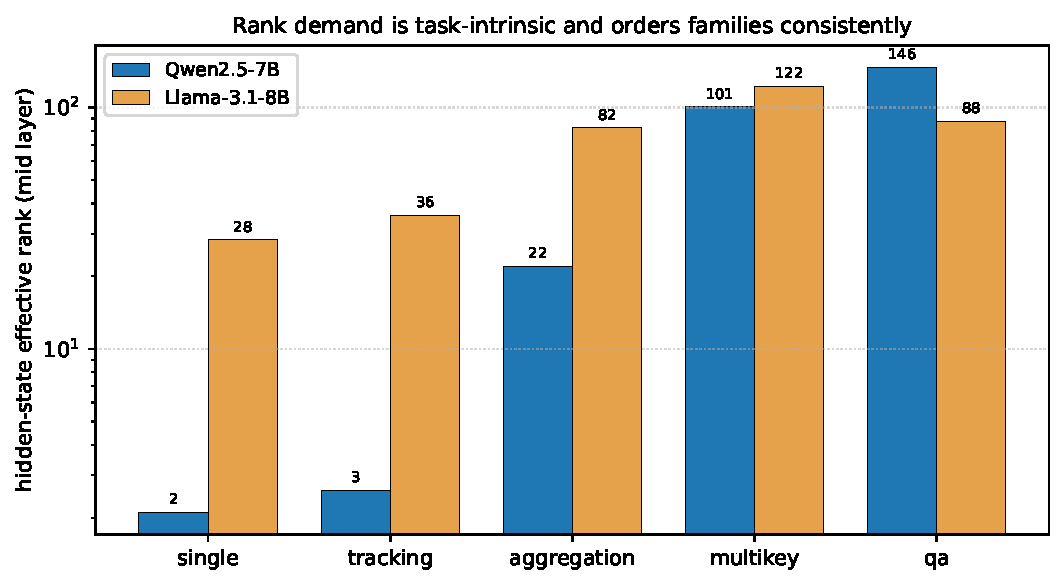
\includegraphics[width=0.72\textwidth]{fig_rank_motivation.pdf}
\caption{Hidden-state effective rank (mid layer, log scale) by RULER task family for both models.
Rank demand is task-intrinsic and orders the families consistently across model families
(qa/multikey high, single/tracking low), yet adds no cross-validated per-sample predictive value
for correctness---motivating the shift from activation space to gradient space.}
\label{fig:rank}
\end{figure}

\section{Conclusion}
\label{sec:conclusion}

We introduced capability fingerprints---CountSketch-compressed per-prompt answer-loss gradients on
a small fixed parameter subset---and showed that the mean fingerprint inner product between a
candidate fine-tuning set and a held-out capability predicts the measured post-fine-tuning change
in that capability's loss, before any training is run. Across four settings (homogeneous
long-context, heterogeneous real skills, a LoRA trainer with disjoint parameters, and a second
model family) the off-diagonal predicted-vs-measured Spearman correlation is $0.68$--$0.87$
(all $p\le0.004$). The ablation localizes the signal to gradient \emph{direction}: magnitude alone
fails in most settings and embedding similarity fails everywhere, sometimes anti-predicting. The
method costs one backward pass and $16$\,KB per prompt and directly supports data selection,
rehearsal targeting, and forgetting-risk assessment.

\paragraph{Limitations.}
Our evaluation uses five capabilities per setting and short fine-tuning horizons ($3$ epochs of
$32$ samples); first-order theory predicts the linear approximation degrades for
longer/higher-learning-rate training, which we have not yet stress-tested. The outcome is
$\Delta$CE; accuracy deltas are noisier at $n_{\text{eval}}=30$. Experiments are at $7$--$8$B
scale on two model families and fp16 Turing hardware, and the parameter subset (q/v of five
layers) is fixed a priori---subset-choice sensitivity is untested.

\paragraph{Future work.}
Natural extensions, currently running, are: capability splits for safety, multilingual, and
reasoning behaviors; horizon scaling (does the first-order prediction decay predictably with
training length?); and rehearsal targeting (selecting data to rehearse by predicted interference
and comparing against random rehearsal). We report these as directions, not results.

\bibliographystyle{iclr2026_conference}
\bibliography{references}

\appendix

\section{Trainer details (fp16 with fp32 masters)}
\label{app:trainer}

All models are served in fp16 on Quadro RTX 8000 (Turing, compute capability 7.5, 48\,GB). Direct
fp16 Adam on the trainable parameters diverges (fp16 rounding of the small Adam updates destroys
the model). Our trainer keeps an fp32 master copy of every trainable parameter; the forward and
backward passes run in fp16 with dynamic loss scaling (scale halved on non-finite gradients,
grown otherwise), gradients are unscaled and cast to fp32, the Adam step is taken on the fp32
masters, and the fp16 weights are refreshed from the masters. Any step with non-finite gradients
after unscaling is skipped. Subset training uses learning rate $2\times10^{-5}$; LoRA (rank $16$,
$\alpha=32$, on all q/v projections) uses $2\times10^{-4}$. Both run $3$ epochs over
$n_{\text{train}}=32$ samples per capability. Weights are restored to the pretrained checkpoint
between capabilities so each $\Delta$CE row is measured against the same reference model.

\section{Hyperparameters and evaluation}
\label{app:hparams}

Per capability: $n_{\text{train}}=32$, $n_{\text{eval}}=30$, seed-disjoint. Sketch dimension
$m=4096$ (one CountSketch $\Phi$ per model, fixed seed, applied per parameter tensor and summed).
Parameter subset $S$: \texttt{q\_proj} and \texttt{v\_proj} at layer-depth fractions
$\{0,\tfrac14,\tfrac12,\tfrac34,1\}$, $\approx 73$M parameters ($105$M for Llama-3.1-8B).
Gradients use teacher-forced
answer cross-entropy with the prompt masked. RULER context length is $1024$ for the interference
experiments and $\{1024,2048,4096,8192\}$ for the rank-demand diagnostic. Correlations are
Spearman and Pearson with two-sided $p$-values; the off-diagonal statistic excludes the five
diagonal (self) cells.

\section{Full measured and predicted matrices}
\label{app:tables}

The complete $5\times5$ measured $\Delta$CE and predicted $-K$ matrices for all four settings are
released in the results files (\texttt{results/interference*/\{measured,predicted\_kernel\}.json}).
The heterogeneous setting is visualized in Figure~\ref{fig:heatmaps}; the remaining settings
follow the same block structure (large negative diagonal, retrieval capabilities weakly coupled).
Accuracy deltas ($\Delta$acc) are recorded alongside $\Delta$CE but are near zero for the
already-saturated retrieval families and noisy for the rest at $n_{\text{eval}}=30$, which is why
$\Delta$CE is the primary outcome.

\end{document}
